\documentclass{article}
\usepackage[utf8]{inputenc}
%\usepackage[catalan]{babel}
\parindent = 0cm %sangria%
\usepackage{amsmath} %Modo matemático%
\usepackage{amssymb,amsfonts,latexsym,cancel}
\usepackage{rawfonts}
\usepackage{pictexwd}
\usepackage{graphicx}  % Para \includegraphics
\usepackage{subcaption} % Para \begin{subfigure}
\usepackage {epstopdf}
\usepackage {float}
\usepackage{amsthm}
\usepackage{centernot}
\usepackage{mathtools}
\usepackage{stmaryrd}
\usepackage {array}
\usepackage {longtable}
\usepackage{enumitem}
\usepackage {bm}
\renewcommand{\baselinestretch}{1.5}
\setlength{\columnsep}{1.75cm}
\usepackage [lmargin=2cm,rmargin=2cm,top=2cm,bottom=2cm]{geometry}
\usepackage{multicol}
\usepackage{paracol}
\usepackage{multirow}
\usepackage{fancyhdr}
\usepackage{url}
\usepackage{braket}
\pagestyle {fancy}
\fancyhead{}
\fancyfoot{}
\fancyhf{}
\fancyfoot{}
\cfoot[\thepage]{\thepage}
\usepackage{amsmath}
\usepackage{float}
\usepackage{hyperref}
\hypersetup{
    colorlinks=true,
    linkcolor=blue,
    filecolor=magenta,      
    urlcolor=cyan,
    }

\usepackage{listings}     % For code listings
\usepackage{color}        % For syntax highlighting colors
\usepackage{xcolor}       % For more color options
\usepackage[T1]{fontenc}  % For special characters (like Å)

% --- Define colors for syntax highlighting ---
\definecolor{codegreen}{rgb}{0,0.6,0}
\definecolor{codegray}{rgb}{0.5,0.5,0.5}
\definecolor{codepurple}{rgb}{0.58,0,0.82}
\definecolor{backcolour}{rgb}{0.95,0.95,0.95}

% --- Configure the 'listings' package for Python ---
\lstdefinestyle{mystyle}{
    backgroundcolor=\color{backcolour},   
    commentstyle=\color{codegreen},
    keywordstyle=\color{blue},
    numberstyle=\tiny\color{codegray},
    stringstyle=\color{codepurple},
    basicstyle=\ttfamily\footnotesize,
    breakatwhitespace=false,         
    breaklines=true,                 
    captionpos=b,                    
    keepspaces=true,                 
    numbers=left,                    
    numbersep=5pt,                  
    showspaces=false,                
    showstringspaces=false,
    showtabs=false,                  
    tabsize=2,
    language=Python,
    frame=single,                   
    rulecolor=\color{black},
    lineskip= 0.5pt,         
    columns=flexible,       
    xleftmargin=2em,        
    framexleftmargin=1.5em, 
    aboveskip=5pt,          
    belowskip=5pt,          
}

\lstset{style=mystyle}

\title{\textbf{Quantum Thermometry}}
\author{Alberto Rodriguez Rodriguez}

\begin{document}
\maketitle
\section{Results that will be used}
For a Gibbs state (system in thermal equilibrium):
\begin{equation}\label{Gibbs operator}
{\varrho}(T) = \frac{1}{Z} \sum_k e^{-\beta \varepsilon_k} |\varepsilon_k\rangle\langle\varepsilon_k|,
\end{equation}
the Quantum Fisher Information (measures of Energy) is given by:
\begin{equation}
    \mathcal{F}(T)=\frac{\Delta^2 H}{T^4}
\end{equation}
So the quantum Cramer-Rao-Bound turns into
\begin{equation}
    \sqrt{\mathcal{N}}\Delta T\geq \frac{1}{\sqrt{\mathcal{F}(T)}}=\frac{T^2}{\Delta H}
\end{equation}
So the main tool used to find optimal or suboptimal thermometers is to optimize(maximize) the energy variance of the diferent systems.
\section{Systems to study}
\subsection{Optimal thermometer - arXiv:1411.2437v3}
\small{\textit{Individual quantum probes for optimal thermometry} (Luis A. Correa, M. Mehboudi, G. Adesso, A. Sanpera)}

\vspace{0.7 cm}
For a general $N$-level probe the energy variance writes as
\begin{equation}\label{Energy Variance}
    \Delta^2 H=\langle H^2\rangle - \langle H \rangle^2=\sum_i^N\varepsilon_i^2 \frac{e^{-\beta\varepsilon_i}}{\mathcal{Z}}-\left(\sum_i^N\varepsilon_i\frac{e^{-\beta\varepsilon_i}}{\mathcal{Z}}\right)
\end{equation}
By imposing $\partial_{\epsilon_i}\Delta^2 H=0$ we obtain the Hamiltonian that maximizes the energy variance
\begin{equation}
    H_{opt} = 0\ket{0}\bra{0} +\sum_i^{D-1}\Omega\ket{i}\bra{i}
    \label{Hopt}
\end{equation}
where the gap has an optimal value (max F.I) when it satisfies the equation
\begin{equation}
    x^*\equiv\frac{\Omega^*}{T}\xrightarrow{}e^{x^*}=(N-1)\frac{x^*+2}{x^*-2}
\end{equation}

\subsection{Suboptimal thermometers with spin networks - arXiv:2211.01934v2}
\small{\textit{Optimal Thermometers with Spin Networks} (P. Abiuso, P.A. Erdman, M. Ronen, F. Noé, G. Haack, M. Perarnau-Llobet)}

\vspace{0.7 cm}
We look for spin networks with 2 body interactions that go as close as they can to the optimal bound. We start with a general hamiltonian 
\begin{equation}
    H = \sum_i^Nh_i\sigma_i^z + \sum_{i<j}^N J_{ij}\sigma_i^z\sigma_j^z
\end{equation}
and again optimize this to obtain the maximum $\Delta^2H$. The optimization is done for $h_i$ and $J_{ij}$. After repeating the optimization for different values of $N$ it was found that for $N \in [2,6]$, the \textit{All-to-All} model performed slightly better than the other system found, the \textit{Star Model}, which becomes the preferred choice for $N \geq 7$. These two systems are described by
\begin{align}
    &H_{Star}(a,b)=a\sigma_1^z + b\sum_{i=2}^{N}\sigma_i^z(\mathbf{I}+\sigma_1^z)
    \label{Hstar}\\
    &H_{all}(h,J)=-h\sum_i^N\sigma_i^z-J\sum_{i<j}^N\sigma_i^z \sigma_j^z
    \label{H_all}
\end{align}

\section{Heat capacity and comparison with optimal bound}
We know heat capacity is closely linked with temperature fluctuations. We can link the Fisher information directly with the heat capacity (at thermal eq and constant volume) of a system through
\begin{equation}
    \mathcal{C}=\frac{\Delta^2H}{T^2}\implies\mathcal{F}(T)=\frac{\mathcal{C}}{T^2}
\end{equation}
For the Optimal system, we can write an explicit expression for this Heat capacity as a function of the gap $x$ and the dimension $D$ of the system:
\begin{align}
    \mathcal{C}_{opt}=e^xx^2\frac{D-1}{(D-1+e^x)^2}
\end{align}
In the asymptotic limit $D\to\infty$ we have
\begin{align}
    \mathcal{C}_{opt}\sim \frac{\ln{D}}{4}
\end{align}
that for a system of $N$ spins, where $D=2^N$, turns into
\begin{align}
    \mathcal{C}_{opt}(2^N)\sim \frac{N^2(\ln2)^2}{4}
\end{align}
So this is the optimal scaling we aim to achieve. For the Star Model, we can compare this behavior in the asymptotic limit:
\begin{equation}
    \mathcal{C}_{star}(2^N)\sim\frac{(N-1)(\ln2)^2}{4}=\mathcal{C}_{opt}(2^{N-1})
\end{equation}
For the All-To-All model this has to be computed numerically.

The comparison between these 3 models gives us the following plot.

\begin{figure}[H]
    \centering
    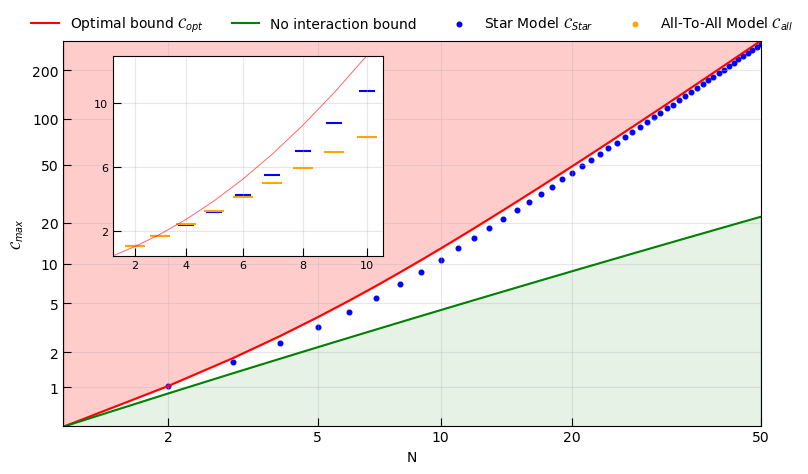
\includegraphics[width=0.9\linewidth]{Cmax(N) (1).png}
    \caption{Maximum Heat capacity as a function of $N$ for the different systems.}
\end{figure}

\section{Thermalization - arXiv:2412.02754v2}
\small{\textit{From dynamical to steady-state many-body metrology: Precision limits and their attainability with two-body interactions}\\Ricard Puig, Pavel Sekatski, Paolo Andrea Erdman, Paolo Abiuso, John Calsamiglia, Martí Perarnau-Llobet}
\vspace{0.7 cm}
Now we are interested in studying the thermalization process of these systems, when they are coupled to a thermal bath. We will restrict ourselves to the conditions of thermalising dynamics, where the evolution of the probabilities of the probe (in its eigenbasis) is given by the master equation
\begin{equation}\label{Pauli Equation}
\frac{d}{dt}P(n,t) = \sum_m \left[ \Gamma_{m\to n} P(m,t) - \Gamma_{n\to m} P(n,t) \right]. 
\end{equation}
Where the transition rates $\Gamma$ must fulfill the detailed balance condition in order to obtain a Gibbs state as the steady solution.

We will also make an extra assumption, that each qubit is locally coupled to a thermal bath, and only transitions between neighboring level can happen. If we define $n$ as the total number of spins up (\textbf{\textit{here is where the problem appears}}), this translates to the equations as
\begin{equation}\label{Probabilities General}
    \dot p_n=-p_n[\Gamma_{n\to n+1}+\Gamma_{n\to n-1}] +p_{n+1}\Gamma_{n+1\to n} + p_{n-1}\Gamma_{n-1\to n}
\end{equation}
Where the rates $\Gamma_{n\to m}$ 
\begin{align}
    &\Gamma_{n\to n+1}=\gamma(N-n)f(\Delta U)\hspace{0.5 cm}; \hspace{0.5 cm}f(\Delta U)=[1+e^{\beta\Delta U}]^{-1}\\
    &\Gamma_{n\to n-1}=\gamma nf(\Delta U)
\end{align}
This is correct for systems that are completely symmetric and states that can be labeled just by the total number of spins up, such as the All-To-All model.

The problem is that, in order to describe with precision the evolution of the probabilities of the Star Model we need to add another label to define the states, to distinguish between the manifold where the center spin is up and another one where it is down (in which all the states have the same energy). This is because the state in which the center spin is down and $k$ spins are up, is also a neighbor of the state with the same number of spins up in the up-manifold. This translates into the probabilities equations as:
\begin{align}
    &\dot{p}(\downarrow, k) = -p(\downarrow, k) \big[ \Gamma_{\downarrow \to \uparrow}(k) + \Gamma_{\downarrow, k \to k+1} + \Gamma_{\downarrow, k \to k-1} \big] + p(\uparrow, k) \Gamma_{\uparrow \to \downarrow}(k) + p(\downarrow, k-1) \Gamma_{\downarrow, k-1 \to k} + p(\downarrow, k+1) \Gamma_{\downarrow, k+1 \to k}\\
    &\dot{p}(\uparrow, k) = -p(\uparrow, k) \big[ \Gamma_{\uparrow \to \downarrow}(k) + \Gamma_{\uparrow, k \to k+1} + \Gamma_{\uparrow, k \to k-1} \big] + p(\downarrow, k) \Gamma_{\downarrow \to \uparrow}(k) + p(\uparrow, k-1) \Gamma_{\uparrow, k-1 \to k} + p(\uparrow, k+1) \Gamma_{\uparrow, k+1 \to k}
\end{align}
The rates now must be treated carefully.

Let's focus first in the satellite spin transitions. The rates for flipping satellites look completely different depending on the central spin. In both cases, if we have $k$ excited satellites out of a total $N-1$ satellites, the combinatorial factors are $(N-1-k)$ for jumping up, and $k$ for jumping down (the same that we had for the all-to-all).

\vspace{0.5 cm}
\textbf{Central spin is $\downarrow$ :} since all states with the central spin down have the exact same energy $E_{down} = -a$, the energy cost to flip any satellite is exactly 0.
\begin{align}
&\textbf{Jump } \mathbf{k \to k+1\,:}\,\Gamma_{\downarrow, k \to k+1} = \gamma (N-1-k) f(0) = \frac{1}{2}\gamma (N-1-k)\\
&\textbf{Jump } \mathbf{k \to k-1\,:}\, \Gamma_{\downarrow, k \to k-1} = \gamma k f(0) = \frac{1}{2}\gamma k\\
&\text{Since } f(0) = 0.5
\end{align}
In this degenerate subspace, the bath just drives purely random, completely unweighted diffusion among the satellites

\textbf{Central spin is $\uparrow$ :} now the satellites feel the field. The energy cost to flip one satellite from down to up:
\begin{align}
&\Delta U_{k\to k+1} = E_{k+1} - E_k = [a + 2b(2(k+1) - N + 1)] - [a + 2b(2k - N + 1)] = 4b\\
&\Delta U_{k\to k-1}=-\Delta U_{k\to k+1}=-4b
\end{align}
So the rates look like
\begin{align}
&\text{Jump } \mathbf{k \to k+1\,:\,} \Gamma_{\uparrow, k \to k+1} = \gamma (N-1-k) f(4b)\\
&\text{Jump } \mathbf{k \to k-1\,:\,} \Gamma_{\uparrow, k \to k-1} = \gamma k f(-4b)
\end{align}
So, now what we have to do is solve the master equations for the probabilities. We can write all these equations together using the Transition matrix formalism
\begin{equation}
    \mathbf{\dot{P}}=M\mathbf{P}
\end{equation}
The first check we can do is to find the steady state via $\mathbf{\dot{P}}=M\mathbf{P}=0$ and compare it with the Gibbs state, to see if the transition matrix is constructed in the right way. We can do this with an easy python code using the function \textit{scipy.linalg.null\_space} that calculates the eigenvectors that have eigenvalue 0.

To solve this, we use the fact that the transition rates/matrix are time independent, so we can simply solve it by
\begin{equation}
    \frac{d\mathbf{P}}{dt}=M\mathbf{P} \xrightarrow{}\mathbf{P}(t)=e^{Mt}\mathbf{P}(0)
\end{equation}
and for each component we have
\begin{equation}\label{pn solutions}
    p_n(t)=\sum_k A_{n,k}\,\,e^{\lambda_k t}
\end{equation}
where $\lambda_k$ are the eigenvalues of the M matrix, and $A_{n,k}$ are coefficients that depend on the initial state and the eigenvectors. 
\newpage
With this last equation we can do our analysis on the thermalization process.

\vspace{0.2 cm}
First, we analyze the thermalization time through the eigenvalue $\lambda_1$, the one with smallest absolute value. Since all the eigenvalues are negative, this $\lambda_1$ will tell us how fast the slowest exponential term vanishes to leave only the steady term.

\vspace{0.2 cm}
Second, we plot how the Fisher Information evolves in time for different values of N. In order to calculate the derivatives of the populations with respect to $\beta$ we have used the numerical derivative around $\beta=1$ with a $\delta \beta=0.001$.

We have the following plots for each model.
\begin{figure}[h!]
    \centering
    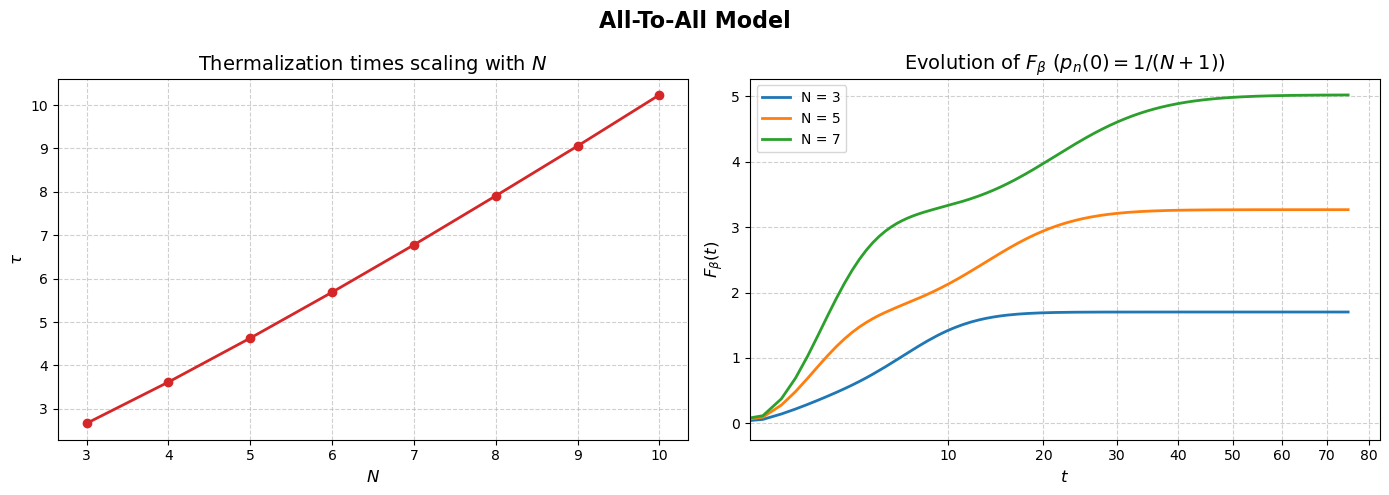
\includegraphics[width=1\linewidth]{ATA_Thermalization.png}
    \caption{Results of the thermalization for the All-To-All model.}
    \label{ATA Thermalization}
\end{figure}

\begin{figure}[h!]
    \centering
    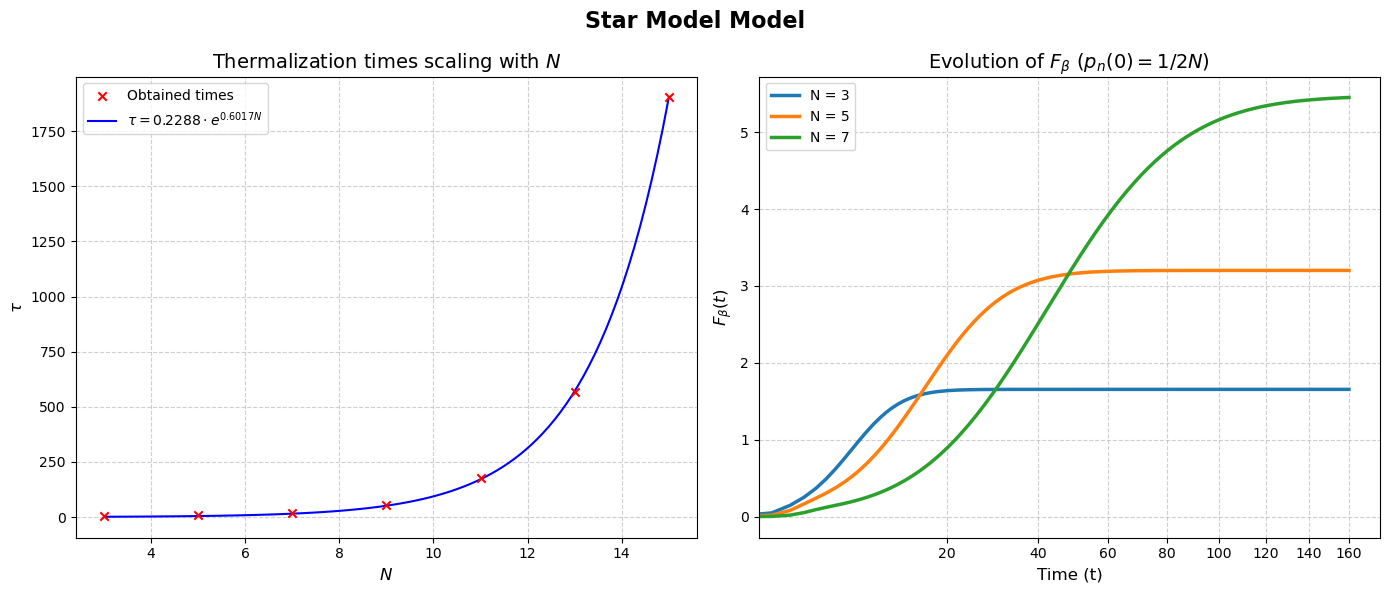
\includegraphics[width=0.99\linewidth]{StarModel_Thermalization.png}
    \caption{Results of the thermalization for the Star Model model.}
    \label{Star Model Thermalization}
\end{figure}

\newpage
So, we have just found the first and most clear trade-off. When we optimize the thermometric precision by increasing the size of the probe we must pay the price of longer thermalization times. Exponential increase for the Star Model and lineal for the All-To-All.

To study the behavior of this trade-off we can use a new figure of merit, we will call it $\chi$ and it is defined as a QFI per unit of time. In equilibrium
\begin{equation}
    \chi_{eq}=\frac{\mathcal{F}_{eq}}{\tau}
\end{equation}

We can analytically predict how this quantity will behave for each model. We know that for the Star Model the FI scales as $\mathcal{F}\sim(N-1)^2$, but its thermalization time scales as $\tau\sim e^N$; but for the All-To-All model they both scale linearly, so:
\begin{align}
    \chi^{Star}_{eq}&=\frac{\mathcal{F}_{eq}}{\tau}\sim\frac{(N-1)^2}{e^N}\xrightarrow{N\gg1}0\\
    \chi^{All}_{eq}&=\frac{\mathcal{F}_{eq}}{\tau}\sim\frac{N}{N}\sim constant
\end{align}
This is shown in this plot
\begin{figure}[H]
    \centering
    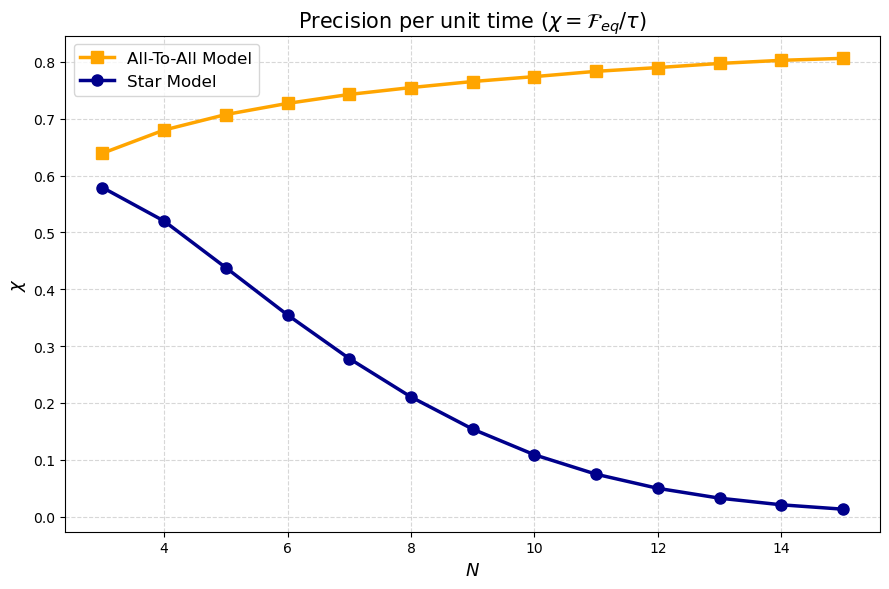
\includegraphics[width=0.54\linewidth]{X_comparison.png}
    \caption{QFI per unit of time comparison between the two models.}
\end{figure}

We can also see the dynamics of this quantity $\chi(t)=\mathcal{F}(t)/t$. From this plot we can select the maximum of this quantity, which could be an interesting point if we want to maximize the QFI but minimizing interaction time too.
\begin{figure}[H]
    \centering
    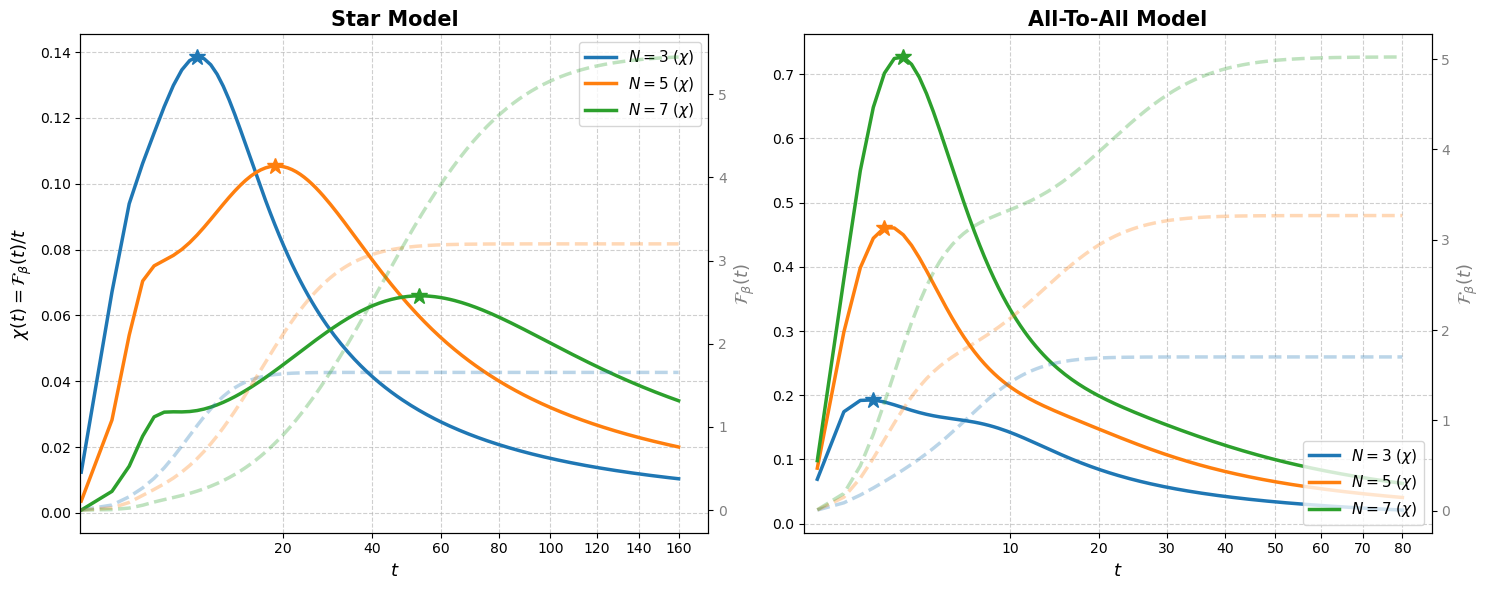
\includegraphics[width=0.9\linewidth]{Dynamical_X_Comparison.png}
    \caption{Dynamical $\chi(t)$ compared to the absolute value of the Fisher Information.}
\end{figure}

\newpage
\section{Next steps}
\begin{itemize}
    \item Find a relation between gaped and exponentially degenerated systems and the exponential scaling of the thermalization time. 
    \item Use the relation of critical exponents:
    \begin{align}
        \mathcal{C}\sim N^{1+\frac{\alpha}{\nu d}}&\\ 
        &\implies \frac{\mathcal{C}}{\tau_{eq}}\sim N^{1+\frac{\alpha-z\nu}{\nu d}}\\
        \tau_{eq}\sim N^{z/d}
    \end{align}
    Try to find systems that satisfy $\alpha - z\nu>0$ and simulate them.
    \item Active quantum control? (Control Hamiltonian Theory) To accelerate or tune thermalization process
\end{itemize}

\newpage

\section{Exponentially scaling thermalization times}
Up to here, we have seen that the Star Model presents a exponential scaling of the thermalization time when we increase the size of the system $N$. In this section, we will try to provide a mathematical proof of this exponential scaling using spectral graph theory, specifically by evaluating the conductance of the Continuous-Time Markov Chain (CTMC) associated with the Pauli master equation.

Let's start by considering the N-level OPTIMAL probe. The system consists of $N$ spins (total dimension $D = 2^N$) governed by a Hamiltonian that yields a single unique ground state and a massively degenerate excited manifold. 

We partition the full state space into two macroscopic sets:
\begin{itemize}
    \item $S$ is the single microstate $|00\dots0\rangle$ with energy $E_0 = 0$ and degeneracy $g_0 = 1$.
    \item $S^c$ are all the other excited states, all with energy $E_1 = \Omega$ and a macroscopic degeneracy of $g_1 = 2^N - 1$.
\end{itemize}

The partition function of the system is given by:
\begin{equation}
    Z = 1 + (2^N - 1)e^{-\beta \Omega}
\end{equation}
and the equilibrium Gibbs probabilities for each macroscopic sets are:
\begin{equation}
    P_{eq}(S) = \frac{1}{Z}\,; \quad \quad P_{eq}(S^c) = \frac{(2^N - 1)e^{-\beta \Omega}}{Z}
\end{equation}

The idea is that the thermalization is dictated by the probability flow between these two sets. Under local thermalizing dynamics (Glauber dynamics), the thermal bath can only induce single-spin flips. So, from the ground state $S$, the system cannot transition to all $2^N - 1$ states in $S^c$ directly. It can only reach the $N$ neighbor states that correspond to only one spin being excited.

Let $\Gamma_{\uparrow}$ be the transition rate for a single spin flip upwards ($\Delta E = \Omega$). The total equilibrium probability flow, we will call it $\mathcal{J}$, escaping the ground state is strictly constrained (o tb li diuen \textit{bottlenecked} x això el concepte) by this physical locality:
\begin{equation}
    \mathcal{J}(S \to S^c) = \sum_{j \in S^c} P_{eq}(S) \Gamma_{0 \to j} = P_{eq}(S) \cdot N \cdot \Gamma_{\uparrow} = \frac{N \Gamma_{\uparrow}}{Z}
\end{equation}

Now, to quantify the metastability of this excited manifold, we calculate the conductance $\Phi(S^c)$. The definition of this quantity is: \textit{"The conductance of a Markov chain, often denoted by $\Phi$ or $\Phi(P)$, measures how quickly the chain converges to its stationary distribution, with higher values indicating faster convergence (rapid mixing) and low values suggesting bottlenecks that trap the chain in subsets of states."} And mathematically it can be calculated as:
\begin{equation}
    \Phi(S^c) = \frac{\mathcal{J}(S \to S^c)}{P_{eq}(S^c)} = \frac{\frac{N \Gamma_{\uparrow}}{Z}}{\frac{(2^N - 1)e^{-\beta \Omega}}{Z}} = \left( \frac{\Gamma_{\uparrow}}{e^{-\beta \Omega}} \right) \frac{N}{2^N - 1}
\end{equation}

By imposing the detailed balance condition, $\Gamma_{\uparrow} P_{eq}(\text{down}) = \Gamma_{\downarrow} P_{eq}(\text{up})$, we can identify the term in parentheses as the rate $\Gamma_{\downarrow}$. So the conductance simplifies to:
\begin{equation}
    \Phi(S^c) = \Gamma_{\downarrow} \frac{N}{2^N - 1}
\end{equation}

For our optimal thermometer, we have seen that the optimal energy gap scales logarithmically with the system size in the asymptotic limit, $\Omega^* \approx T \ln(N)$. This tells us that for standard physical environments the transition rate $\Gamma_{\downarrow}$ will scale at most logarithmically or polynomially with $N$, but no exponentially.

Now we use the 2nd and most important tool, to Cheeger's inequality, it says that: \textit{the mixing time $\tau$ of a reversible Markov chain is strictly bounded from below by the inverse of the system's conductance}:
\begin{equation}
    \tau \ge \frac{1}{2\Phi(S^c)} = \frac{2^N - 1}{2 N \Gamma_{\downarrow}(N)}
\end{equation}

Since the entropic bottleneck in the numerator grows exponentially as $2^N = e^{N \ln 2}$, and the physically allowed transition rates in the denominator can only grow logarithmically ($\Gamma_{\downarrow} \propto \ln N$), the thermalization time is strictly bounded by:
\begin{equation}
    \tau \ge \mathcal{O}\left( \frac{e^{N \ln 2}}{N \ln N} \right)
\end{equation}

This result matches the observed scaling for the Star Model too!!!. So we have just seen that mathematically any optimal thermometric probe exhibiting an exponentially growing density of states will have the price of an exponentially long thermalization time under local dynamics. The bath cannot provide transition rates large enough to overcome the metastable ''entropic bottleneck'' created by the $2^N$ state space.

\section{Generalization for any \{$E_n,g_n$\}}

Up to here, we established an analytical bound showing that maximizing the energy variance (and thus the heat capacity $\mathcal{C}$) requires a highly degenerate excited manifold, and this specific topology forces an exponential slowdown in the thermalization time $\tau$. Now we have related this thermalization time with an ``entropic bottleneck'', that emerges because of the physical constraints of local bath interactions and the high density of states. 

Given this trade-off, we can ask the following question: instead of evaluating predetermined microscopic models (Star, All-To-All, optimal...), can we find the absolute optimal spectrum that maximizes the precision per unit time, $\chi = \mathcal{C}/\tau$? To answer this, we shift from forward analysis to inverse design, optimizing a generic $n$-level macroscopic system.

To start, we consider a generalized system defined by $n$ macroscopic energy levels. Each level $i \in \{1, 2, \dots, n\}$ is characterized by an energy $E_i$ and a macroscopic degeneracy $g_i$. To map this back to an $N$-spin equivalent system, we impose the global Hilbert space constraint:
\begin{equation}
    \sum_{i=1}^{n} g_i = 2^N, \quad \text{with} \quad 0 = E_1 \le E_2 \le \dots \le E_n
\end{equation}
The thermodynamic quantities, such as the partition function $Z$ and the heat capacity $\mathcal{C}$, can be easily computed from these macroscopic parameters. However, evaluating the dynamical timescale $\tau$ requires constructing the $n \times n$ transition rate matrix $M$.

The difficult part comes when we try to find a general way to describe $\tau$, in such a way it can be optimized or calculated in a numerical way. It can be done, but we need to make an assumption over the microscopic transitions network. A general transition rate, under Glauber framework, can be written as:
\begin{equation}
    \Gamma_{i \to j} = \gamma\frac{K_{ij}}{g_i} \frac{1}{1 + e^{\beta(E_{j} - E_i)}}
\end{equation}
where $K_{ij}$ is defined as the conductivity, and is where the dynamics/interactions/system topology is encoded. It describes the number of paths/ways that connect the two subspaces involved in the transition. For example in the All-To-All model, the number of connections between a level with $k$ spins up and a level with $k+1$ is exactly $K_{k,k+1}=\binom{N}{k}\times(N-k)$.

This makes us to make a decision, we need to ''impose'' some conditions on the system in order to optimize the figure of merit, or maybe go through another direction?

Options go keep going:
\begin{itemize}
    \item Impose different $K_{ij}$ to see the optimal \{$E_n,g_n$\} for each system, and try to see if there is any general behavior?\\
    \item Instead of optimize over macroscopic variables \{$E_n,g_n$\}, start with the general Hamiltonian again
        \begin{equation}
            H = \sum_{i} B_i \sigma_z^i + \sum_{i < j} J_{ij} \sigma_z^i \sigma_z^j
        \end{equation}
    and optimize $B_i$ and $J_{ij}$ (computationally harder)
\end{itemize}
    

\newpage
\section*{Papers}

An information-theoretic proof of the Planckian bound for thermalization -  arXiv:2506.19188v1 \\

Thermometry in the quantum regime: Recent theoretical progress - arXiv:1811.03988v3 \\

Optimal nonequilibrium thermometry in Markovian environments - arXiv:2107.04425v2\\

Quantum thermometric sensing: Local vs. Remote approaches - arXiv:2510.16628v1\\

Thermodynamic Geometry Through Second Order Phase Transitions - arXiv:2512.01936v1\\

Quantum Gibbs Samplers: the commuting case - arXiv:1409.3435v3\\

The power of a critical heat engine - arXiv:1603.05024v2\\

Minimizing Dissipation via Interacting Environments: Quadratic Convergence to Landauer Bound - arXiv:2411.00944v1\\



\end{document}
